%\chapter{The Optimum Receiver}

\subsection{RC Circuit}
%
\begin{problem}
Refer to the circuit in Fig. \ref{fig:2.1}. Suppose you are told that $C$ has a resistance given by $\frac{1}{s  C}$.   Find the ratio $H(s)$ of the output voltage and input voltage using node analysis.  The above circuit is known as a low pass filter and $H(s)$ is known as the transfer function.
\end{problem}
%
%
\begin{figure}[!h]
\centering
\includegraphics[width=\columnwidth]{./chapter2/figs/2.1.eps}
%\vspace*{-13cm}
\caption{Three stage $R-C$ low pass filter circuit}
\label{fig:2.1}
\end{figure}
%

\solution The equations at the nodes are given by
%
\begin{align}
\frac{V_1-V_i}{R}+ {sCV_1} + \frac{V_1-V_2}{R} &= 0
\\
\frac{V_2-V_1}{R}+ {sCV_2} + \frac{V_2-V_o}{R} &= 0
\\
\frac{V_o-V_2}{R}+ {sCV_o} &= 0
\end{align}
%
which can be expressed as
%
\begin{equation}
\begin{pmatrix}
sC + \frac{2}{R} & -\frac{1}{R} & 0 
\\
-\frac{1}{R}  & sC + \frac{2}{R} & -\frac{1}{R}
\\
0 & -\frac{1}{R} & sC + \frac{1}{R} 
\end{pmatrix}
\begin{pmatrix}
\frac{V_1}{V_i}
\\
\frac{V_2}{V_i}
\\
\frac{V_o}{V_i}
\end{pmatrix}
= 
\begin{pmatrix}
\frac{1}{R}
\\
0
\\
0
\end{pmatrix}
\end{equation}
%
Thus,
\begin{align}
H(s) &= \frac{V_o}{V_i} = 
\frac{
\begin{vmatrix}
sC + \frac{2}{R} & -\frac{1}{R} & \frac{1}{R}
\\
-\frac{1}{R}  & sC + \frac{2}{R} & 0
\\
0 & -\frac{1}{R} & 0
\end{vmatrix}
}{
\begin{vmatrix}
sC + \frac{2}{R} & -\frac{1}{R} & 0 
\\
-\frac{1}{R}  & sC + \frac{2}{R} & -\frac{1}{R}
\\
0 & -\frac{1}{R} & sC + \frac{1}{R} 
\end{vmatrix}
}
\\
&= \frac{1/R^3}{\brak{sC + \frac{1}{R} }\cbrak{\brak{sC + \frac{2}{R} }^2-\frac{1}{R^2}}-\frac{1}{R^2}\brak{sC + \frac{2}{R} }}
\end{align}
%
which can be expressed as
%
\begin{align}
H(s) &= \frac{1}{\brak{sCR + 1 }\cbrak{\brak{sCR + 2 }^2-1}-\brak{sCR + 2 }}
\\
&= \frac{1}{\brak{sCR + 2 }^3 - \brak{sCR + 2 }^2 - 2\brak{sCR + 2 } + 1}
\\
&= \frac{1}{\brak{sCR}^3 - 5 \brak{sCR }^2 + 6sCR  + 1}
\label{lpf_laplace}
\end{align}
%
\begin{problem}
Substitute $s = \j 2\pi f, \j =  \sqrt{-1}$ in \eqref{lpf_laplace} to obtain $H(f)$.  $H(f)$ is known as the frequency response. Plot $\abs{H(f)}$ in octave for $-20 < f < 20$, given that $R = 1 \,k\Omega$ and $C = 10 \,\mu F$.
\end{problem}
%
\solution 
%
Type  the following code to get Fig. \ref{fig:filter_plot}.  You will find that $H(f)$ is a low pass
filter.
%
\lstinputlisting[language=octave]{./chapter2/codes/2.2.py}
%
\begin{figure}[!h]
\centering
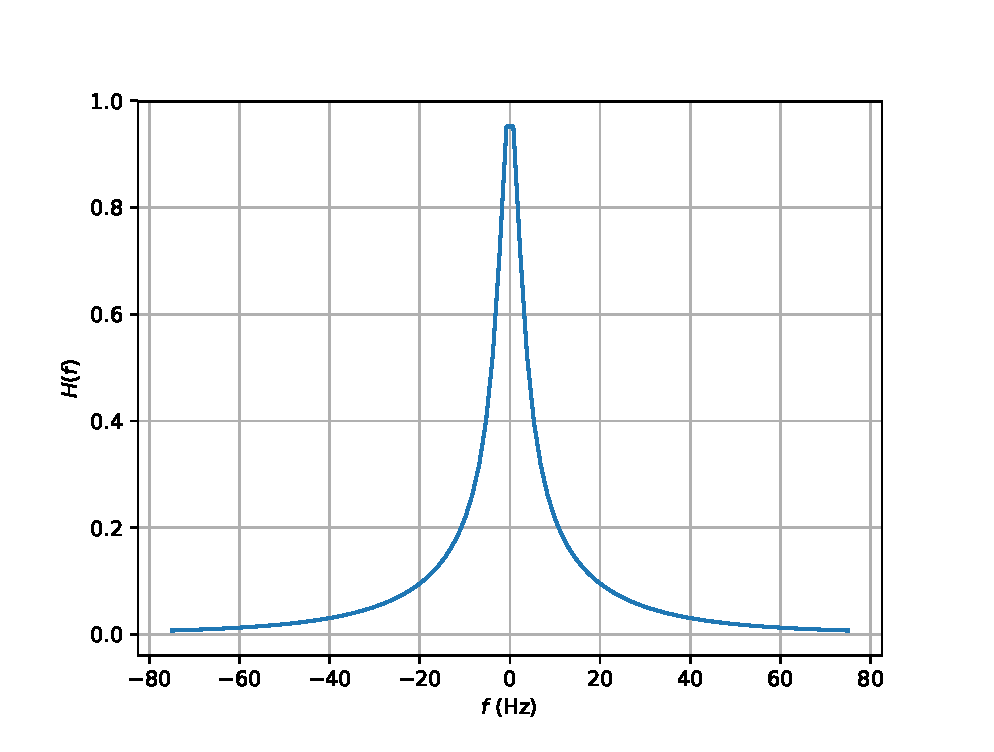
\includegraphics[width=\columnwidth]{chapter2/figs/2.2.eps}
%\vspace*{-13cm}
\caption{Frequency response of the $R-C$ filter}
\label{fig:filter_plot}
\end{figure}
\begin{problem}
Find the frequency at which $\abs{H(f)}^2 = \frac{1}{2}$. This frequency is
known as the 3-dB bandwidth of $H(f)$.
\end{problem}
%
\solution Substituting sCR = \j x in \eqref{lpf_laplace},
%
\begin{align}
 \abs{H(\j x)} &= \frac{1}{\sqrt{2}} \\
 \Rightarrow 
 -jx^3 + 5x^2 +j6x + 1 &= \sqrt{2} \\
\Rightarrow 
 x^2(6-x^2)^2 + (1+5x^2)^2 &= 2 \\
 \Rightarrow 
x^6 + 13x^4 + 46x^2 -1&= 0 
\end{align}
%
Letting $y=x^2$, we obtain the cubic equation
%
\begin{align}
y^3 + 13y^2 + 46 y -1 = 0
\end{align}
%
The following script gives the 3 dB bandwidth for the filter H by choosing the 
real root.
%
\lstinputlisting[language=octave]{./chapter2/codes/2.3.py}
%
This yields the value $f_{3\, dB} = 2.3395$ Hz.
\begin{problem}
Obtain the 3 dB bandwidth by solving the cubic equation in the previous problem
\end{problem}
%
\solution In the above, let $y = z - \frac{13}{3}$.  Then the equation becomes
%%
\begin{align}
\Rightarrow z^3 - (31/3)z  -1015/27  & = 0
\end{align}
%%
This equation has the theoretical solution evaluated by the following script
%
\lstinputlisting[language=octave]{./chapter2/codes/2.4.py}
Note that this script gives the same result as the one in the previous problem.
%Let
%%
%\begin{equation}
%\begin{split}
%q &= -31/3\\
%r &= -1135/9
%\end{split}
%%
%\end{equation}
%%
%Then
%%
%\begin{align}
%y = \cbrak{-\frac{r}{2} + \sqrt{\frac{r^2}{4} + \frac{q^3}{27}} }^{\frac{1}{3}} + \cbrak{-\frac{r}{2} - \sqrt{\frac{r^2}{4} + \frac{q^3}{27}} }^{\frac{1}{3}} - \frac{13}{3}
%\end{align}
%%
%and
%%
%\begin{align}
%x = \sbrak{\cbrak{-\frac{r}{2} + \sqrt{\frac{r^2}{4} + \frac{q^3}{27}} }^{\frac{1}{3}} + \cbrak{-\frac{r}{2} - \sqrt{\frac{r^2}{4} + \frac{q^3}{27}} }^{\frac{1}{3}} - \frac{13}{3}}^{\frac{1}{2}}
%\end{align}
%
\begin{problem}
\label{filter_op}
Suppose the square wave in Fig. \ref{fig:1.1} is given as input to the filter in Fig. \ref{fig:filter_plot}.  Find and plot the filter output.
\end{problem}
%
\solution  Using sinusoidal steady state analysis, if the input to the filter is
%
$\cos{2\pi n f t}$, the output is given by
\begin{equation}
\abs{H(nf)}\cos\cbrak{2\pi n f t + \angle H(nf)}
\end{equation}
%
Using the principle of superposition, for the input 
%
\begin{equation}
\sum_{n=0}^{\infty}a_n\cos 2\pi n f t + b_n \sin 2 \pi n f t
\end{equation}
%
the output will be
%
%
\begin{multline}
\sum_{n=0}^{\infty}a_n\abs{H(nf)}\cos\cbrak{2\pi n f t + \angle H(nf)} 
\\
+ b_n \abs{H(nf)}\sin\cbrak{2\pi n f t + \angle H(nf)}
\end{multline}
%
Suitably modifying the program in Problem \ref{fourier_series},
%
\lstinputlisting[language=python]{./chapter2/codes/2.5.py}
%
The output of the filter is shown  in Fig. \ref{fig:2.5}
\begin{figure}[!h]
\centering
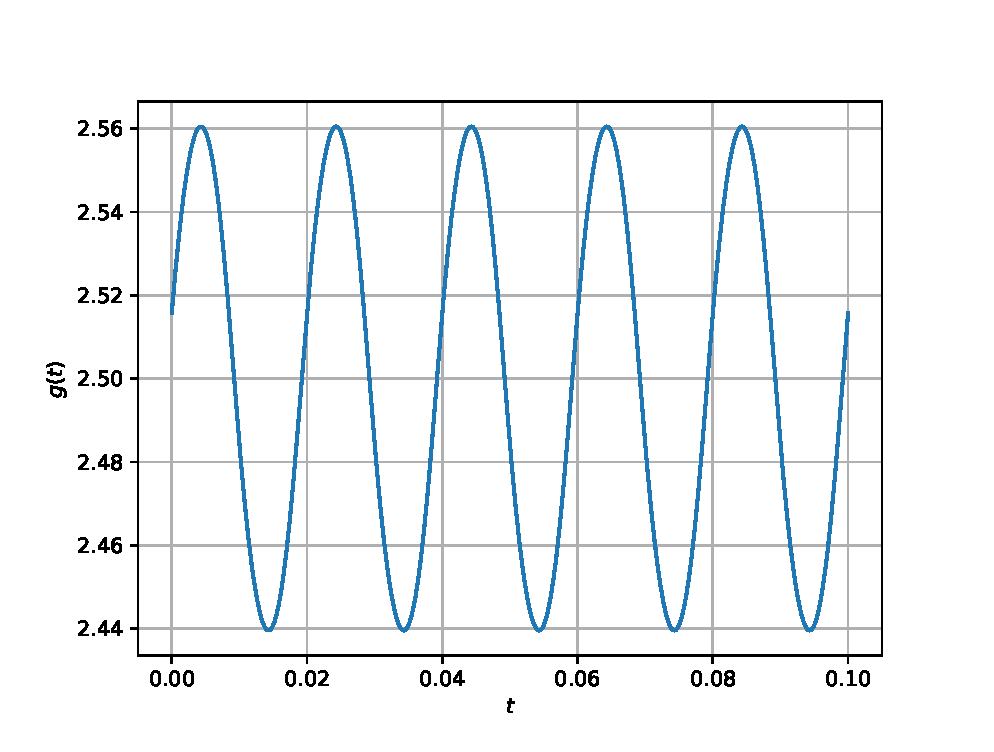
\includegraphics[width=\columnwidth]{./chapter2/figs/2.5.eps}
%\vspace*{-13cm}
\caption{Output of the $R-C$ filter}
\label{fig:2.5}
\end{figure}
%
\begin{problem}
Run the program in problem \ref{filter_op} by changing the for loop to
\begin{verbatim}
for n in range(2):
\end{verbatim}
Compare this output with the one in Fig. \ref{fig:2.5} by plotting in the same graph.
\end{problem}
\begin{problem}
Interpret the result in problem \ref{filter_op}.
\end{problem}
%
\solution
In Fig. \ref{fig:filter_plot}, $\abs{H(0)} = 1$ and $\abs{H(50)} = 0.02$.  All other values of $H$ are very small.  $\abs{H(0)} = 1$ contributes the DC component and $\abs{H(50)} = 0.02$ yields the sinusoidal component of 50 Hz.  Thus, $H(f)$ filters all higher harmonics in the square wave in Fig. \ref{fig:1.1}.
%\begin{problem}
%Sketch $\abs{H(nf)}$.
%\end{problem}
%%
%\solution
%\lstinputlisting[language=octave]{./chapter2/codes/2.6.m}
%%
%The output of the filter is shown  in Fig. \ref{fig:2.6}
%\begin{figure}[!h]
%\centering
%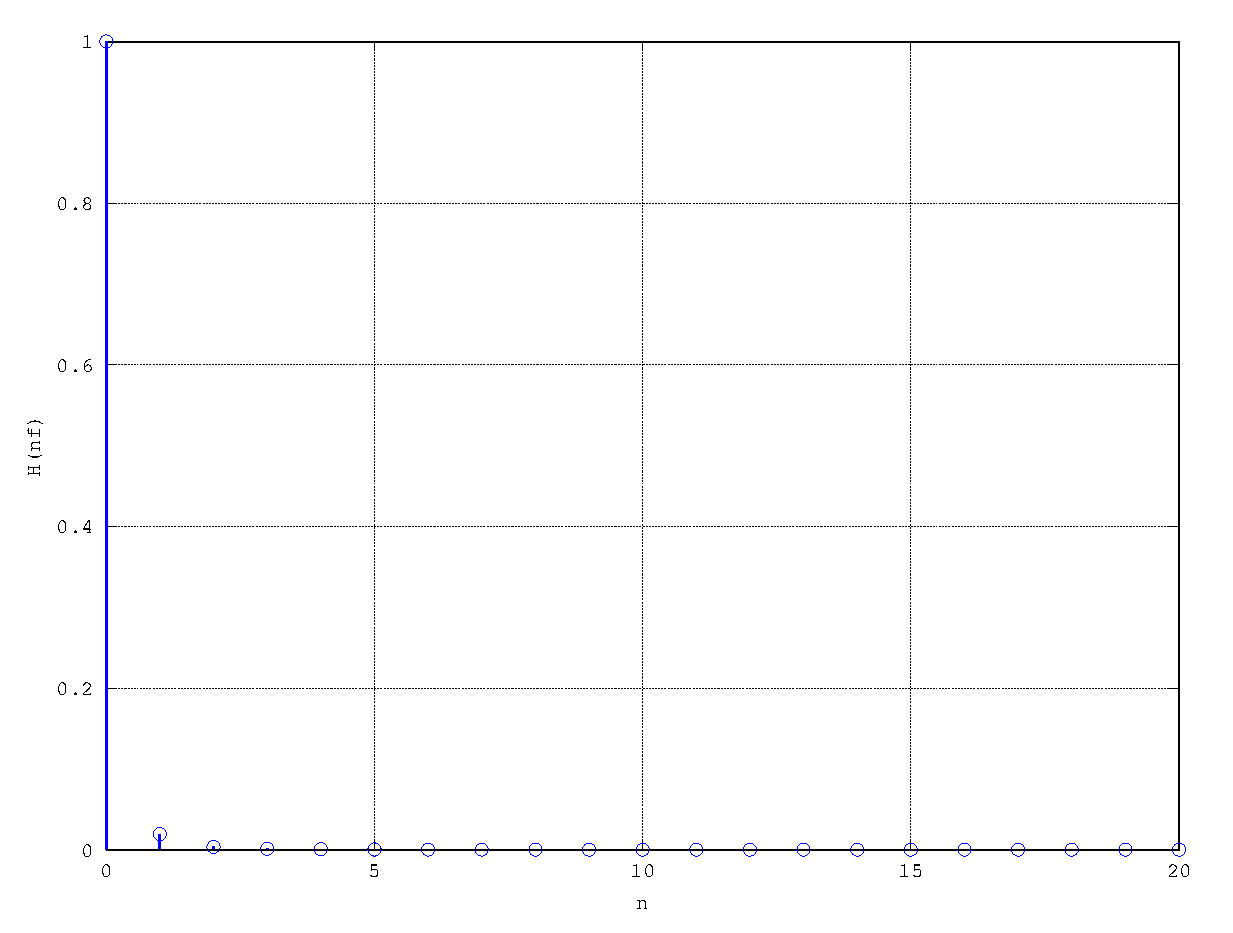
\includegraphics[width=\columnwidth]{./chapter2/figs/2.6.eps}
%%\vspace*{-13cm}
%\caption{Frequency response of the $R-C$ filter}
%\label{fig:2.6}
%\end{figure}
%%

%\begin{problem}
%Connect $g(t)$ to the following circuit for $R = 10 \,k \Omega, C = 10 \,\mu F$ and observe the output $v(t)$.  Measure the amplitude and time period of $v(t)$.
%\end{problem}
%\subsection{Circuit Analysis}
%%
%\begin{problem}
%	Obtain the expression for $H(s)$ using mesh analysis.
%\end{problem}
%%
%\begin{problem}
%	Repeat the above exercise using Thevenin's theorem.
%	\end{problem}
%	%
%	\begin{problem}
%		Repeat the above exercise using Norton's theorem.
%		\end{problem}
%	%
%	\begin{problem}
%		Repeat the above exercise using $Y-\Delta$ transformation.
%	\end{problem}
%\begin{problem}
%	Obtain all the two port network parameters for the circuit in Fig. \ref{fig:2.1}.
%\end{problem}
%			
%\begin{problem}
%For $R = 10 \,k \Omega, C = 1 \,\mu F$, plot $H(f)$ with respect to $f$.  Comment.
%\end{problem}
%\subsection{RL Circuit}
%%
%\begin{problem}
	%Using node analysis, design an $R-L$ circuit with the same frequency response as the $R-C$ circuit in the previous section.  Comment.
%\end{problem}
%%
%\begin{problem}
%Obtain the frequency response for this $R-L$ circuit using mesh analysis.
	%\end{problem}
	%%
%\begin{problem}
%Repeat the above exercise using Thevenin's theorem.
%\end{problem}
		%%
		%\begin{problem}
%Repeat the above exercise using Norton's theorem.
			%\end{problem}

%\subsection{Bandpass Filter}
%%
%\begin{problem}
	%Design an $R-C$ bandpass filter  and use it to filter a higher harmonic from the square wave generated using the arduino.
%\end{problem}
%%
%\begin{problem}
%Obtain the frequency response of the above filter.
%\end{problem}
%%
%\begin{problem}
%Obtain the above frequency response using an $RLC$ circuit.
%\end{problem}
%
